\chapter{Introducción} \chapterlabel{Informe/1-Introduccion} \label{cap:Introducción}

\noindent Actualmente, los sistemas que emplean levitación magnética son de gran interés debido a que ofrecen la posibilidad de reemplazar algunos sistemas mecánicos con la gran ventaja de que reducen significativamente las pérdidas de energía ocasionadas por el roce, además de ser más suaves y menos ruidosos. 

\noindent Una de las aplicaciones  más importantes que tiene la levitación magnética es en trenes que utilizan este fenómeno para guiarse e impulsarse, comúnmente conocidos como ``MagLev''. Los vagones levitan sobre la vía mediante una fuerza magnética de atracción generada por electroimanes colocados en su parte inferior, como se  observa en la figura \ref{fig:img_tren}. Debido a la alta inestabilidad que presenta el fenómeno de levitación magnética, es necesario utilizar un sistema de control que mantenga constante la distancia sobre la que se mantiene suspendido.

\begin{figure}[H]
	\centering
	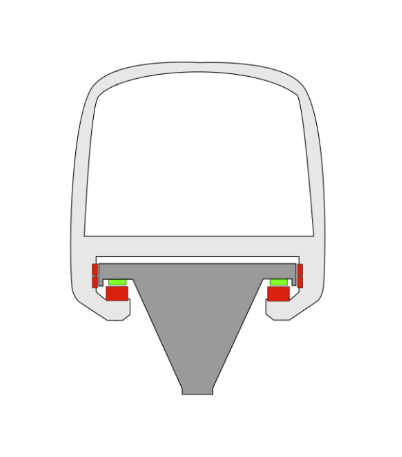
\includegraphics[scale = 0.85]{tren.png}
	\caption{Aplicación de levitación magnética.}
	\label{fig:img_tren}
\end{figure}

\noindent El desarrollo del sistema de levitación magnética planteado para este proyecto surge como idea de la cátedra Sistemas de Control de la carrera de Ingeniería Electrónica. Su objetivo es disponer de una planta de control con la  que se puedan realizar prácticas en clase. Una primera versión de este dispositivo fue diseñada y construida por la cátedra. Los desarrolladores de este proyecto tuvieron la oportunidad de realizarle pruebas y modificaciones durante el cursado de la asignatura. Sin embargo, no se pudo lograr que funcionara correctamente al finalizar la cursada. Por este motivo, se propuso hacer una revisión y rediseño de todas las etapas que componen al sistema en el marco de un proyecto final.

Desde el punto de vista de la asignatura Sistemas de Control, es de interés el estudio y experimentación con un sistema de levitación magnética ya que integra varios conceptos dictados durante la cursada y otros aprendidos en el transcurso de la carrera. En principio se puede mencionar que este tipo de sistemas presentan un alto grado de inestabilidad, por lo que es necesario el diseño de un compensador adecuado. La planta presenta un comportamiento no lineal con respecto a la variable de control y a la variable que se desea controlar. Además, se implementa una fuente de corriente conmutada que permite trabajar con corrientes elevadas al mismo tiempo que se minimizan las pérdidas de energía.

\section{Alcance del proyecto}

\noindent El objetivo de este proyecto es realizar un modelado teórico de un sistema de levitación magnética a partir de un electroimán de laminación normalizada con núcleo tipo “E''. Este integra las etapas de \textsl{driver} de corriente de potencia, estimación de distancia de levitación, y control de la planta. Estas dos últimas se implementan tanto en forma analógica como digital.

\noindent Este documento contempla el proceso de diseño y modelado de todas las etapas pertenecientes al sistema, junto con su implementación circuital y simulaciones. Además, se realiza el diseño del circuito impreso de la placa de control.



\section{Contexto del proyecto}

\noindent El proyecto comenzó a desarrollarse en junio del 2020. Inicialmente tenía como objetivo el diseño y la construcción de un prototipo funcional que permitiera a los alumnos de la asignatura de Sistemas de Control realizar mediciones y observar el comportamiento de las distintas etapas que componen el sistema. Sin embargo, debido a los retrasos ocasionados por la pandemia (COVID-19), los costos asociados a la fabricación de la placa de control y sus componentes, sumado a la  necesidad de no extender indefinidamente el proyecto, se optó por acotar el alcance sólo al modelado teórico de todas las etapas y al diseño del circuito impreso.

\noindent Se espera que en el futuro se pueda construir el sistema de levitación magnética para que sirva como herramienta para los alumnos, de forma tal que les permita experimentar y afianzar los conceptos teóricos adquiridos durante el transcurso de la cursada.



\section{Descripción del dispositivo}

\noindent El dispositivo está compuesto por dos partes principales: un electroimán y una placa de control. El electroimán tiene dos piezas formadas por láminas de acero apiladas: una con forma de “E”, que tiene un cable bobinado en su rama central y otra con forma de “I” que es atraída por la primera mediante una fuerza electromagnética. Esta fuerza es regulada por la placa de control, que mantiene la distancia de separación ($Y_{g}$) o \textsl{gap} de aire deseado entre ellas mientras que el objeto que se desea hacer levitar se sujeta de la pieza en forma de “I”. Dicha separación puede ser modificada por el usuario entre $3\:mm$ y $5\:mm$ y el peso máximo que se puede hacer levitar es de $30\:kg$. El sistema completo se muestra en la figura \ref{fig:img_Esquema-del-producto}.

\begin{figure}[H]
	\centering
	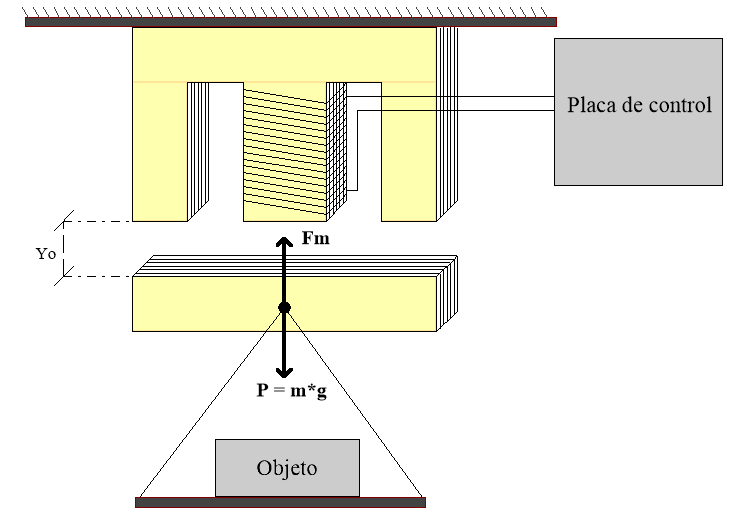
\includegraphics[width=\textwidth]{esquema-del-producto.png}
	\caption{Esquema del dispositivo.}
	\label{fig:img_Esquema-del-producto}
\end{figure}


La placa de control actúa sobre la fuerza magnética que ejerce el electroimán para compensar las perturbaciones que pueda recibir el sistema y mantener constante la separación $Y_{g}$. Solo puede ejercer control de la posición sobre el eje vertical, por lo que las desviaciones de posición en el eje horizontal no pueden ser controladas y pueden provocar un comportamiento no deseado.

El sistema de control está conformado por las etapas que se muestran en la figura \ref{fig:img_diagrama-en-bloques-del-sistema}. Integra dos controladores distintos: uno analógico y otro digital. Cada uno de ellos se compone de un compensador y un estimador de posición.  El usuario decide cual de estas implementaciones ejerce el control mediante la utilización de un \textsl{switch}, por lo que solo una estará activa al mismo tiempo. El sistema analógico está formado por un circuito de  componentes pasivos y amplificadores operacionales, mientras que el digital está basado en un microcontrolador re-programable.

\begin{figure}[H]
	\centering
	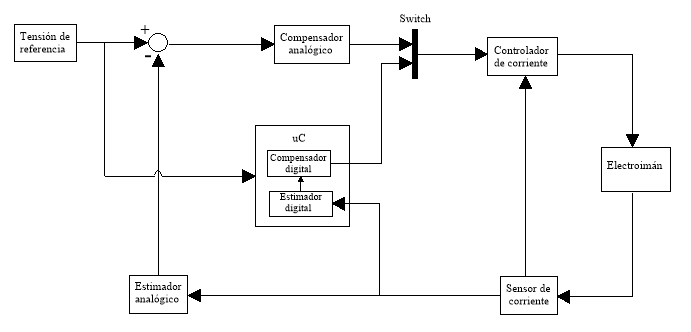
\includegraphics[width=\textwidth]{diagrama-en-bloques-del-sistema.png}
	\caption{Diagrama en bloques del sistema.}
	\label{fig:img_diagrama-en-bloques-del-sistema}
\end{figure}

\noindent El estimador de posición se encarga de entregar una tensión proporcional al \textsl{gap} de aire real a partir de la corriente que circula por el electroimán. El usuario puede modificar el \textsl{gap} según desee al variar la tensión entregada por un potenciómetro presente en la placa de control. Tanto la implementación analógica como la digital reciben esta entrada que es comparada con la estimación y luego, su resultado, es utilizado como entrada para el compensador.

Debido a que la planta es naturalmente inestable, se utiliza un compensador para lograr la estabilidad y la distancia de separación deseada. En su entrada recibe la comparación de la referencia de posición con la estimación y en base a ella modifica la corriente que ingresa al electroimán, y por ende la fuerza que este ejerce.

El controlador de corriente cumple la función de adaptar los niveles de tensión de salida del compensador a niveles de corriente aptos para que el electroimán genere la fuerza suficiente para sostener el objeto que se hace levitar.
 